\documentclass{article}

\title{Mini-project: Evil Toddlers and Stone Fruit}
\author{Henry Oehlrich \and Jo Coimbatore \and Noah Curtis}

\usepackage[margin=1.25in]{geometry}
\usepackage{pgfplots}
\usepackage{pgfplotstable}
\usepackage{pgf-pie}
\usepackage{caption}
\usepackage{subcaption}
\usepackage{booktabs}

\pgfplotsset{compat=1.18}
\pgfplotstableread[row sep=\\,col sep=&]{
    Do you know what a stone fruit is? & Number of evil toddlers \\
    Yes & 5.857 \\
    No & 23.304 \\
}\fruitandtoddlers
\usepgfplotslibrary{statistics}
\captionsetup[figure]{labelfont={bf}}

\begin{document}
\maketitle

Two Google Form surveys were sent out through email on September 7, 2023 and
September 8, 2023 to the second and third period Raleigh Charter High School AP
Statistics classes. These two surveys asked students a total of 23 quantitative
and qualitative questions, and a total of 34 answers were collected. We decided
to compare the data collected from the questions, “Do you know what a stone
fruit is?” and “How many evil toddlers could you beat in a fight?” We thought
these questions would be interesting to analyze because we were curious to see
if there was any relationship between knowledge of a term used in real life and
confidence in a hypothetical fight.

Before analyzing the data, it was first refined. The form allowed for any text
entry so there were some responses that were not simply numbers. The change in
the data is shown in Figure \ref{fig:data}. Entries that were removed are
bolded and the entry that was changed is italicized. For all of our analyses,
we use the modified data shown in Figure \ref{subfig:modified}.

% Five number summaries
\begin{figure}[ht]
    \centering
    \caption{Five number summaries}
    \label{fig:fivenum}
    \begin{tabular}{l|l|l|l|l|l|l}
        \toprule
        Conditional & Min & Q1 & Median & Q3 & Max & IQR \\
        \midrule
        All & 0 & 2 & 5 & 20 & 100 & 18 \\
        Stone fruit & 0 & 2 & 5 & 7 & 20 & 5 \\
        No stone fruit & 0 & 2 & 5 & 20 & 100 & 18 \\
    \end{tabular}
\end{figure}

% Box plot
\begin{figure}[ht]
    \centering
    \caption{Box plots}
    \label{fig:boxplots}
    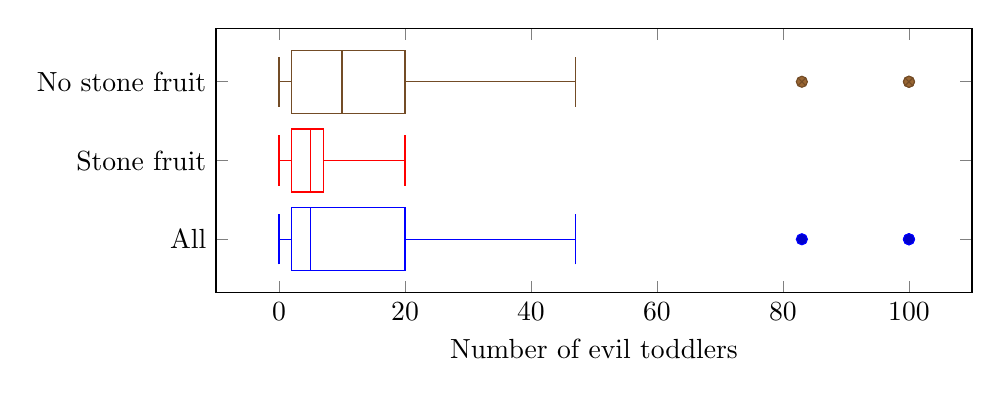
\begin{tikzpicture}
        \begin{axis}[
                y=1cm,
                x=0.08cm,
                ytick={1,2,3},
                yticklabels={All, Stone fruit, No stone fruit},
                xlabel={Number of evil toddlers},
            ]
            \addplot+ [
                boxplot prepared={
                    lower whisker=0,
                    lower quartile=2,
                    median=5,
                    upper quartile=20,
                    upper whisker=47,
                },
            ] table [row sep=\\,y index=0] {
                data\\ 100\\ 100\\ 83\\
            };
            
            \addplot+ [
                boxplot prepared={
                    lower whisker=0,
                    lower quartile=2,
                    median=5,
                    upper quartile=7,
                    upper whisker=20,
                },
            ] coordinates {};

            \addplot+ [
                boxplot prepared={
                    lower whisker=0,
                    lower quartile=2,
                    median=10,
                    upper quartile=20,
                    upper whisker=47,
                },
            ] table [row sep=\\,y index=0] {
                data\\ 100\\ 100\\ 83\\
            };
        \end{axis}
    \end{tikzpicture}
\end{figure}

The five number summaries in Figure \ref{fig:fivenum} are represented in the
boxplots in Figure \ref{fig:boxplots}. These graphs show that those who are
familiar with stone fruits tend to be less confident in their abilities against
evil toddlers than their less knowledgeable counterparts. The boxplots also
clearly show the outliers in the data. It is also clear that all outliers occur
in the group of people who are not familiar with stone fruits.

\newpage

% Bar chart
\begin{figure}[ht]
    \centering
    \caption{Bar chart of number of evil toddlers by knowledge of stone fruits}
    \label{fig:fruitandtoddlers}
    \begin{tikzpicture}
        \begin{axis}[
                width=1\textwidth,
                height=.5\textwidth,
                ymin=0,
                ymax=30,
                ylabel={Number of evil toddlers},
                xtick=data,
                xticklabels from table={\fruitandtoddlers}{Do you know what a stone fruit is?},
                xlabel={Do you know what a stone fruit is?},
                ybar,
                bar width=-.5,
                ybar=1pt,
                enlarge x limits={abs=0.5},
            ]
            \addplot table [x expr=\coordindex, y=Number of evil toddlers]{\fruitandtoddlers};
        \end{axis}
    \end{tikzpicture}
\end{figure}

The bar chart in Figure \ref{fig:fruitandtoddlers} reinforces the idea that
those who are familiar with stone fruits report that they could take less evil
toddlers in a fight than those who are not familiar with stone fruits. It is
prudent to note that the bar chart above shows the \textit{average} number of
evil toddlers fought. This is because the number of students who reported they
did not know what a stone fruit is was much larger than the number of students
who reported they did know what a stone fruit is. The pie chart in Figure
\ref{fig:stonefruitpie} shows the distribution of stone fruit knowledge.

% Pie chart
\begin{figure}[ht]
    \centering
    \caption{Pie chart of stone fruit knowledge}
    \label{fig:stonefruitpie}
    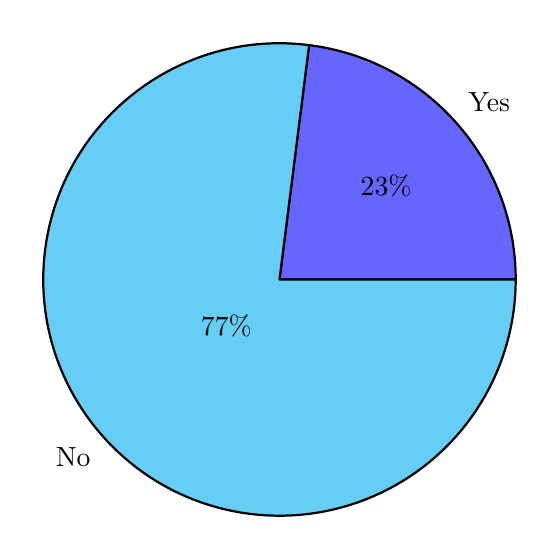
\begin{tikzpicture}
        \pie{23/Yes, 77/No}
    \end{tikzpicture}
\end{figure}

\newpage

% Histogram
\begin{figure}[ht]
    \centering
    \caption{Histogram of number of evil toddlers}
    \label{fig:toddlershist}
    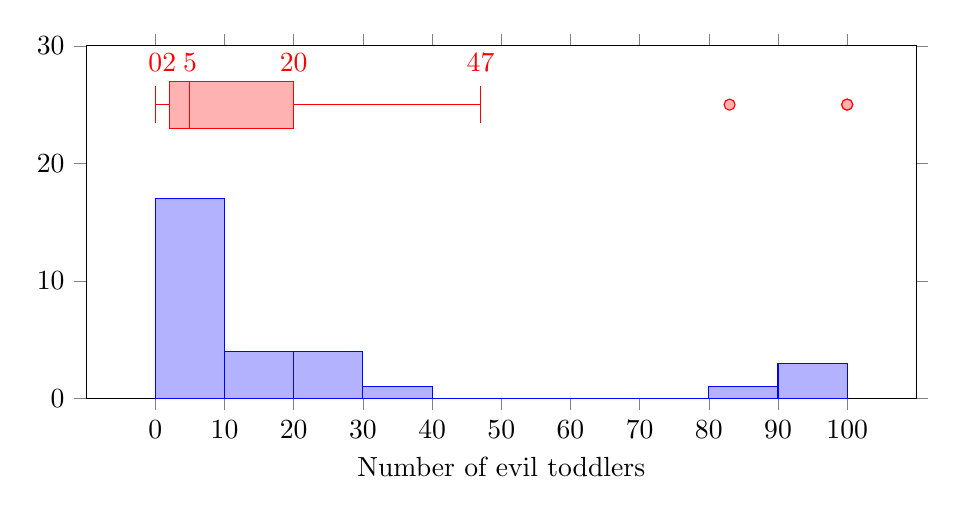
\begin{tikzpicture}
        \begin{axis}[
                width=1\textwidth,
                height=.5\textwidth,
                ymin=0,
                ymax=30,
                xlabel={Number of evil toddlers},
                %xmin=0,
                %xmax=100,
                xtick=data,
                ybar,
                tick align=outside,
            ]
            \addplot+[hist={bins=10}]
            table [row sep=\\,y index=0] {
                data\\
                10\\ 20\\ 20\\ 5\\ 2\\ 1\\ 20\\ 1\\ 100\\ 0\\ 100\\ 2\\ 2\\
                0\\ 5\\ 10\\ 2\\ 3\\ 100\\ 30\\ 3\\ 15\\ 2\\ 0\\ 0\\ 7\\
                10\\ 4\\ 83\\ 20\\
            };
            \addplot+[
                boxplot prepared={
                    draw position=25,
                    box extend=4,
                    lower whisker=0,
                    lower quartile=2,
                    median=5,
                    upper quartile=20,
                    upper whisker=47,
                },
            ] table [row sep=\\, y index=0 ] {
                data\\ 100\\ 100\\ 83\\
            } 
            [above]
            node at
                (boxplot box cs: \boxplotvalue{lower whisker},1)
                {\pgfmathprintnumber{\boxplotvalue{lower whisker}}}
            node at
                (boxplot box cs: \boxplotvalue{lower quartile},1)
                {\pgfmathprintnumber{\boxplotvalue{lower quartile}}}
            node at
                (boxplot box cs: \boxplotvalue{median},1)
                {\pgfmathprintnumber{\boxplotvalue{median}}}
            node at
                (boxplot box cs: \boxplotvalue{upper quartile},1)
                {\pgfmathprintnumber{\boxplotvalue{upper quartile}}}
            node at
                (boxplot box cs: \boxplotvalue{upper whisker},1)
                {\pgfmathprintnumber{\boxplotvalue{upper whisker}}}
            ;
        \end{axis}
    \end{tikzpicture}
\end{figure}

The histogram in Figure \ref{fig:toddlershist} shows the distribution of the
number of evil toddlers students reported they could beat in a fight. The
distribution is unimodal and skewed to the right. It's center is from 2 to 20,
but the boxplot clearly shows that the data are most concentrated between 2 and
5. Even after removing the most extreme outliers, the distribution still
contains multiple outliers.

\begin{figure}[ht]
    \centering
    \caption{Contingency table of stone fruit knowledge and favorite Backyardigan character}
    \label{fig:contingency}
    \begin{tabular}{l|l|l|l|l|l|l}
        \toprule
        & Never watched & Uniqua & Pablo & Tyrone & Tasha & Total\\
        \midrule
        Yes & 2 & 4 & 1 & 0 & 0 & 7 \\
        No & 10 & 5 & 6 & 5 & 2 & 28 \\
        Total & 12 & 9 & 7 & 5 & 2 & 35 \\
    \end{tabular}
\end{figure}

You guys let me know what to put here

% Data
\begin{figure}
    \centering
    \caption{Data}
    \label{fig:data}
    \begin{subfigure}{.5\textwidth}
        \centering
        \caption{Original Data}
        \label{subfig:original}
        \begin{tabular}{p{3cm}|p{3cm}}
            \toprule
            Know stone fruit? & \# evil toddlers \\
            \midrule
            No & 10 \\
            Yes & 20 \\
            No & 20 \\
            Yes & 5 \\
            Yes & \bf{maaaaaybe 2} \\
            No & 1 \\
            No & 20 \\
            No & 1 \\
            No & 100 \\
            No & 0 \\
            No & 100 \\
            No & 2 \\
            No & 2 \\
            No \\
            Yes & 0 \\
            No & \bf{500} \\
            Yes & 5 \\
            No & 10 \\
            No & 2 \\
            No & 3 \\
            No & 100 \\
            No & 30 \\
            No & 3 \\
            No & 15 \\
            No & \bf{haven't tested it} \\
            Yes & 2 \\
            No & \textit{0 tbh (I'm a pacifist)} \\
            No & 0 \\
            Yes & 7 \\
            No & 10 \\
            No & \bf{I might not be sure on that} \\
            No & 4 \\
            No & \bf{1000} \\
            No & 83 \\
            No & 20 \\
        \end{tabular}
    \end{subfigure}%
    \begin{subfigure}{.5\textwidth}
        \centering
        \caption{Modified Data}
        \label{subfig:modified}
        \begin{tabular}{p{3cm}|p{3cm}}
            \toprule
            Know stone fruit? & \# evil toddlers \\
            \midrule
            No & 10 \\
            Yes & 20 \\
            No & 20 \\
            Yes & 5 \\
            No & 1 \\
            No & 20 \\
            No & 1 \\
            No & 100 \\
            No & 0 \\
            No & 100 \\
            No & 2 \\
            No & 2 \\
            Yes & 0 \\
            Yes & 5 \\
            No & 10 \\
            No & 2 \\
            No & 3 \\
            No & 100 \\
            No & 30 \\
            No & 3 \\
            No & 15 \\
            Yes & 2 \\
            No & 0 \\
            No & 0 \\
            Yes & 7 \\
            No & 10 \\
            No & 4 \\
            No & 83 \\
            No & 20 \\
        \end{tabular}
    \end{subfigure}%
\end{figure}

\end{document}
